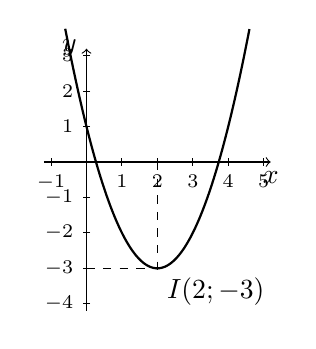
\begin{tikzpicture}[scale=0.45]
    \draw[->] (-1.2,0) -- (5.2,0) node[below] {$x$};
    \draw[->] (0,-4.2) -- (0,3.2) node[left] {$y$};

    \foreach \x in {-1,1,2,3,4,5}
        \draw (\x,0.1) -- (\x,-0.1) node[below] {\scriptsize $\x$};

    \foreach \y in {-4,-3,-2,-1,1,2,3}
        \draw (0.1,\y) -- (-0.1,\y) node[left] {\scriptsize $\y$};

    \draw[smooth, samples=200, domain=-0.6:4.6, thick]
        plot (\x, {\x*\x - 4*\x + 1});

    \fill (2,-3) circle (1.3pt);
    \draw[dashed] (2,0) -- (2,-3);
    \draw[dashed] (0,-3) -- (2,-3);
    \node[below right] at (2,-3) {$I(2;-3)$};
\end{tikzpicture}
